\documentclass[11pt]{article}
\usepackage{amssymb}
\usepackage{amsmath}
\usepackage{semantic}
\usepackage{listings}
\usepackage{hyperref}
\usepackage{graphicx}
\usepackage{algpseudocode}


\title{Evolution of ORM Systems: Formal Foundations}
\author{Ondrej Macek}

\begin{document}
\tableofcontents \newpage

\maketitle
\begin{abstract}
The formal definition of the evolution in context of  software created using an object oriented programming language and a relational database is introduced in this paper. Special attention is given to the data stored in databases (instances) and theirs consistency during evolution process.
\end{abstract}

\textbf{Keywords:} data evolution, data migration
\section{Introduction}
The evolution of an application is a common issue during software development. The evolution can occur from many reasons in different parts of application lifecycle. The evolution of a software  created using an object oriented programming language and a relational database is usually processed as code refactoring and database migration is processed as a set of SQL scripts. The code refactoring is supported by many IDEs and the database migration is supported by many frameworks and tools, nevertheless these tools are usually not capable to solve complicated migration cases or preserve stored data. Another disadvantage is the evolution has to be define twice - as a code refactoring and as a database migration.

This paper provides a formal description of an evolutionary framework, which evolves a database including stored data according to a evolution in application. There are defined models representing an application and database in the paper, together with functions which are able to perform an evolution of the whole software.

The paper is organized as follows: in Section \ref{sec:evolution} the concept of ORM software and its evolution is discussed, then models of application and database are introduced in Section \ref{sec:appModel} and in Section \ref{sec:dbModel}, the ORM is defined in Section \ref{sec:orm} and the evolutionary transformations are defined in Section \ref{sec:eorm}.

\section{Data Evolution in ORM Software}
\label{sec:evolution}
The ORM software consist of an application created using object oriented language and relational database. The application and database are in consistent state according to a concrete ORM function, otherwise the software cannot work properly. An ORM software is illustrated in Figure \ref{fig:appStructure}. The software can be defined as a triple:
\begin{equation*}
	software = < Application, Database, \rho >
\end{equation*}
Models of $Application$ and $Database$ will be introduced in detail in Section \ref{sec:appModel} and in Section \ref{sec:dbModel}, the ORM function $\rho$ is defined in Section \ref{sec:orm}. The consistent state of application and database is defined as:
$$\rho(Application) = Database$$
 
\begin{figure}
\begin{center}
	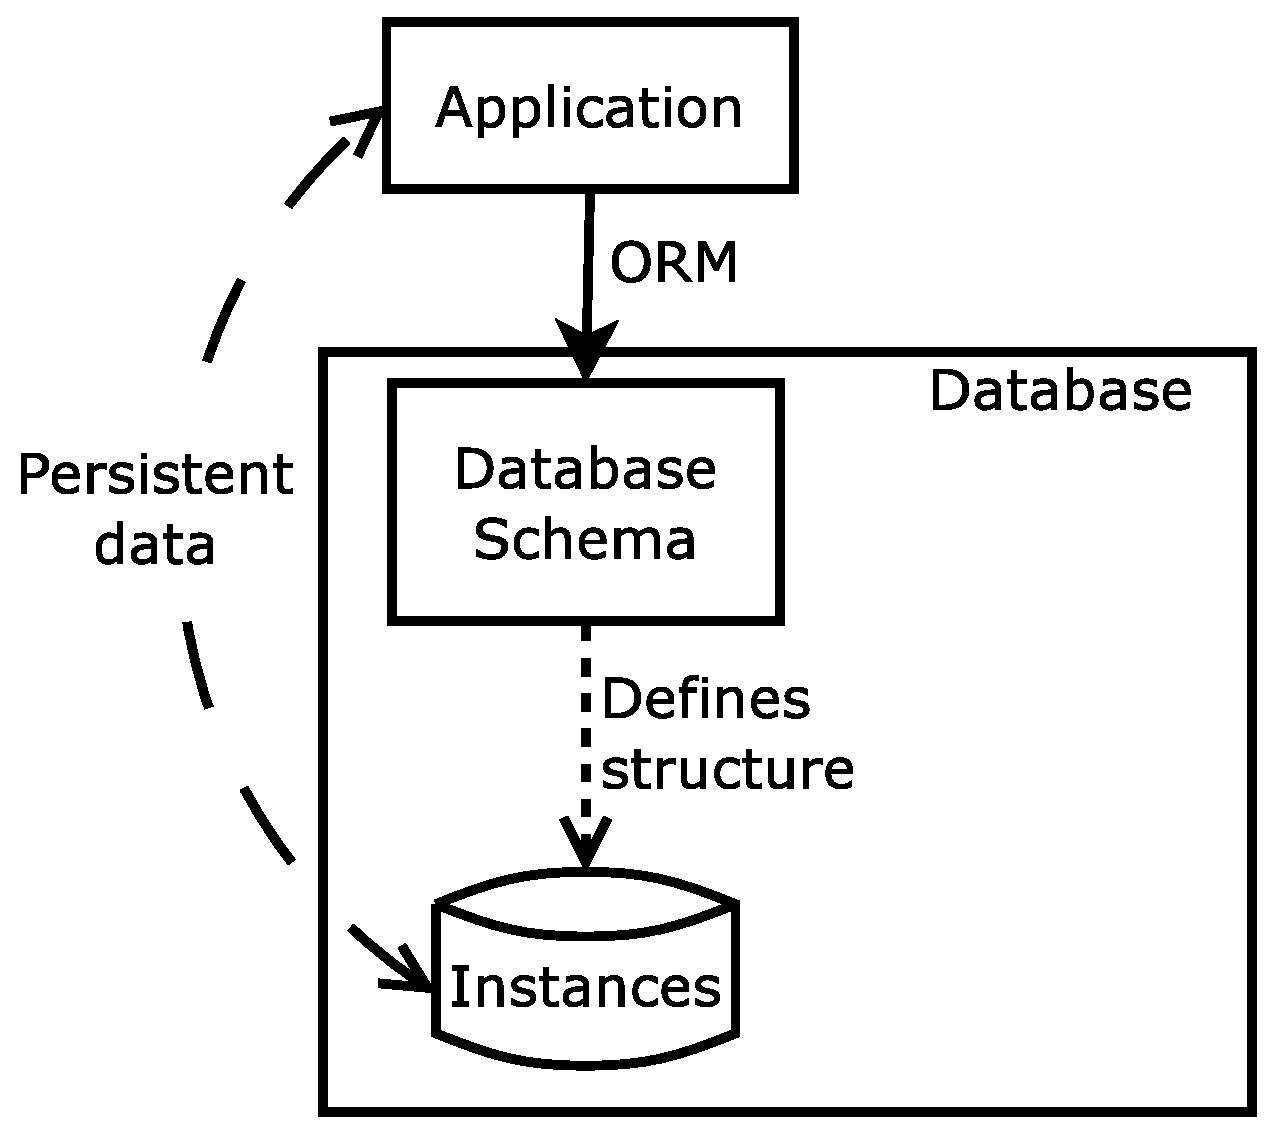
\includegraphics[scale=0.3]{./images/system}
	\caption{The model of one generation of an ORM system consists of application persistent layer and relational database for storing instances.}
\end{center}
	\label{fig:appStructure}
\end{figure}

The evolution of an software is a transformation of one consistent state to another consistent state: $$\epsilon : system \rightarrow system $$ We will call consistent states of one software \emph{generations} of the software. The evolution is quite easy if we consider only structure of an application and database and ignore instances (stored data). The evolution can be described in such a case as:
\begin{equation*}
\epsilon(software(App, Db)) = \{a \rightarrow \epsilon_{App}(App)  | software(a, \rho(a), \rho)\}
\end{equation*}
It means only the structure of the application is evolved and the new database is obtained as a result od ORM. Stored data are usually useless in many cases as their structure does not correspond to the new database schema. We believe the data preservation and consistency is a crucial issue during the software evolution. 

The evolution process we propose is in Figure \ref{fig:evolution}. The transition from the first generation to the second one is based on application evolution which is interpreted on the database level. The interpretation of application evolution is called evolutionary object-relation mapping (eORM) and its defined as a function:
\begin{equation*}
	\Phi : \epsilon_{app} \rightarrow \epsilon_{db}
\end{equation*}
The evolution of the software can be than defined as:
\begin{equation*}
\epsilon(software(App, Db)) = \{software(\epsilon_{app}(App), \Phi((\epsilon_{app}, Db), \rho)\}
\end{equation*}


\begin{figure}
\begin{center}
	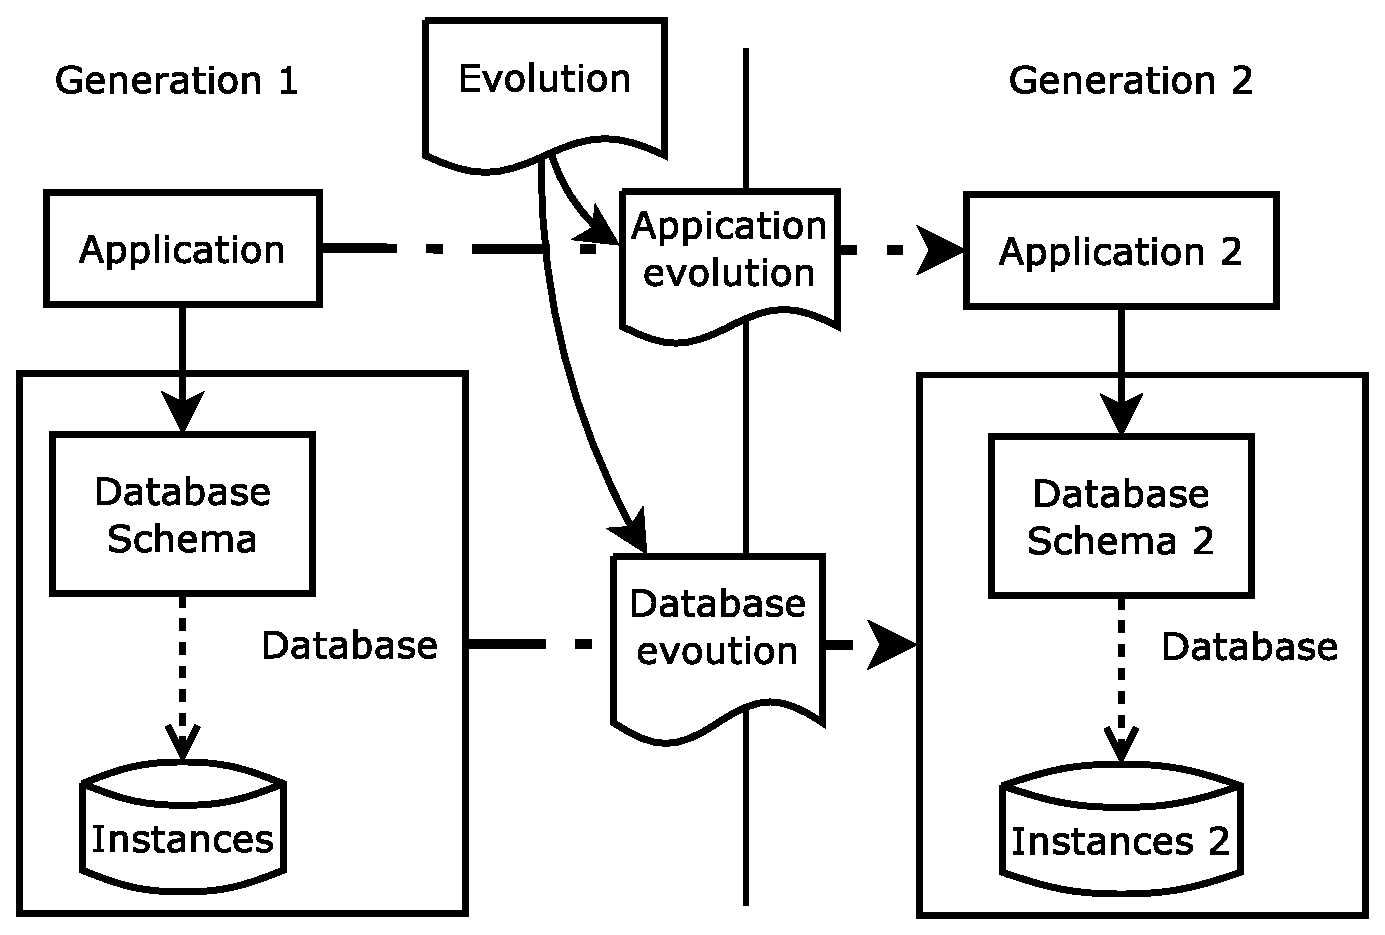
\includegraphics[scale=0.4]{./images/evolution_simple}
	\caption{The evolution of data changes the system on all levels. The figure shows all the components of the evolution process.}
\end{center}
	\label{fig:evolution}
\end{figure}


\begin{itemize}
	\item \textbf{TODO state monade}
\end{itemize}


\section{Application Model}
\label{sec:appModel}
The model represents a persistent layer of an application created using object oriented language. It means the layer is a set of instances which cooperates together. Each instance is defined according to a class - the class defines the structure and relationships of the instance. The instances are stored in the relational database in our case, therefore we define only the structure of classes in our model. 

The model uses a set $Labels$ which contains all possible identifiers for the model. Each model component which has a label ($label \in Labels$) is unambiguously identified in the model.
 
$$
Application = < Class* > 
$$
$classes : Application \rightarrow Class*$ \\
$classes(<cs, is >) = cs, cs \in Class* \wedge is \in Instance* $ \\ \\
$class : Label \times Application \rightarrow Class  $ \\ 
$class(l, a) = c, c \in classes(a) \wedge name(c) = l, l \in Label, a = Application $ \\ \\
The structure of an application consists not only of classes, it is defined by five other concepts. Besides the structure definition, there is defined a set of functions, which allows to manipulate the application model easily. 

\paragraph{Class} represents a basic structural concept in the application model. It has a unique name, one or more properties and a class can be associated to other classes in the application. 
	 
$$Class = < label, Property*, Association* >$$
$name : Class \rightarrow Label$ \\
$name(< lab, props, assocs  >) = lab$ \\ \\
$properties : Class \rightarrow Property*$ \\
$properties(< lab, props, assocs  >) = props $\\ \\
$primitiveProperties : Class \rightarrow Property*$ \\
$primitiveProperties(< lab, props, assocs  >) = props', \forall p \in props' : cardinality(p) \leq 1 $\\ \\
$collectionProperties : Class \rightarrow Property*$ \\
$collectionProperties(< lab, props, assocs  >) = props', \forall p \in props' : cardinality(p) > 1 $\\ \\
$associations : Class \rightarrow Association*$ \\
$associations(< lab, props, assocs  >) = assocs $ \\ \\
$associated :  Class \times Application \rightarrow Boolean $
%TODO: variable types

\paragraph{Property} represents a feature of  a class which is can be represented as a primitive type. The property can be mandatory, can have a default value.
$$
Property = < label, AppType, DefaultValue, Cardinality, Mandatory >
$$
$name : Property \rightarrow Label$ \\
$name(< lab, t, val, n  >) = lab$ \\ \\
$type : Property \times AppType$ \\
$type(< lab, t, val, n  >) = t$ \\ \\
$cardinality : Property \rightarrow NzNat$ \\
$cardinality(< lab, t, val, n  >) = n$ \\ \\
$mandatory : Property \rightarrow Boolean $
$mandatory(<lab, t, val, n, m >) = = m $ \\ \\
$owningClass : Property \times Application \rightarrow Class $ \\
$owningClass(p, a) = c, c \in classes(a) \wedge p \in properties(c) $
%TODO: variable types

\paragraph {Association} represents a connection between two classes. It has a unique name and it contains a name of the class which is referenced by the association. The class which owns the association is consider to be a starting class of an association, referenced class is consider to be an ending class of an association. The cardinalities defines the multiplicity of the association.
$$
Association = (label, classRef, startCardinality, endCardinality)
$$
$name : Association \rightarrow Label$ \\
$name(< lab, ref, n_1, n_2  >) = lab$\\ \\
$reference : Association \rightarrow Label$ \\
$reference(< lab, ref, n_1, n_2  >) = ref$\\ \\
$startCardinality : Association \rightarrow NzNat$ \\
$startCardinality(< lab, ref, n_1, n_2  >) = n_1$\\ \\
$endCardinality : Association \rightarrow NzNat$ \\
$endCardinality(< lab, ref, n_1, n_2  >) = n_2$ \\ \\
$owningClass : Association \times Application \rightarrow Class $ \\
$owningClass(as, a) = c, c \in classes(a) \wedge as \in associations(c) $
%TODO: variable types

\paragraph{AppType} represents primitive types in the application. There are usually defined types such as String, Integer, Boolean etc. in contrast there is only one type in our model, because we focus on structural and data changes and type casting operations are not important for us. The only App-Type type is called APP-STRING.
$$
AppType = APPSTRING
$$
The types used in application model:
$$
cardinality = NzNat
$$
$$
referencesClass = label
$$
$$
startCardinality = NzNat
$$
$$
endCardinality = NzNat
$$

%%%%%%%%%%%%%%%%%%%

\section{Database Model}
\label{sec:dbModel}
The relational database consists of database schema which defines the structure of the database and data, which in our ORM system represents instances. The database is:
$$
Database = <table*, row*>
$$
$table : Label \times Database \rightarrow Table $ \\
$table(l, d) = t, t \in tables(d) \wedge name(t) = l$ \\

\subsection{Database Schema Model}
The database schema model is defined by following concepts:
\paragraph{Table} represents a basic concept of database schema. It has a unique name, one or more column and it can be related to other tables in the schema by foreign keys. Rows in the table represents stored data.
$$
Table = (label, primaryKey, Column*, ForeignKey*)
$$
$name : Table \rightarrow Label $ \\
$name(< lab, pk, cols, fks  >) = lab$ \\ \\
$primaryKey : Table \rightarrow PrimaryKey $ \\
$primaryKey(< lab, pk, cols, fks  >) = pk$ \\ \\
$columns : Table \rightarrow Column* $ \\
$columns(< lab, pk, cols, fks  >) = cols$ \\ \\
$foreignKeys : Table \rightarrow ForeignKey* $ \\
$foreignKeys(< lab, pk, cols, fks  >) = fks$ 

\paragraph{Column} columns define possible data values and types which can be part of a table record.
$$
Column = (label, DbType, DefaultValue, Constraint*)
$$
$name : Column \rightarrow Label $ \\
$name(< lab, t, val, cons  >) = lab $ \\ \\
$type : Column \rightarrow DbType $ \\
$type(< lab, t, val, cons  >) = t $ \\ \\
$constraints : Column \rightarrow Constraint* $ \\
$constraints(< lab, t, val, cons  >) = cons $ \\ \\
$owningTable : Column \times Database \rightarrow Table $ \\
$constraints(c, d) = tab, tab \in tables(d) \wedge c \in columns(d) $

\paragraph{Foreign key}
$$
ForeignKey = (label, tableRef, Constraint*)
$$
$name : ForeignKey \rightarrow Label $ \\
$name(< lab, tRef, cons  >) = lab $ \\ \\
$reference : ForeignKey \rightarrow Label $ \\
$reference(< lab, tRef, cons  >) = tRef $ \\ \\
$reference : ForeignKey \rightarrow Constraint* $ \\
$reference(< lab, tRef, cons  >) = cons $ \\ \\
$owningTable : ForeignKey \times Database \rightarrow Table $ \\
$owningTable(fk, d) = tab, tab \in tables(d) \wedge fk \in foreignKeys(d) $

\paragraph{Primary key}
$$
PrimaryKey =  < label > 	
$$

\paragraph{DbType} represents primitive types in the database. There are usually defined types such as Char, Integer, Boolean etc. There is only one type defined in the model which is called DBSTRING.
$$
DbType = DBSTRING
$$

\paragraph{Constraint} there are two types of constraints defined in the model. Both constraints are column constraints - first constraint defines unique records in a column, second constraint defines non-empty columns.

\begin{center}
$Constraint = NOTNULL$ $|$ $UNIQUE $
\end{center}

\subsection{Model of Stored Data}





A row in a table is tuple consisting of reference to a concrete table and a set of value pairs, which represents concrete values of concrete columns.
$$row = < refTable, pair* >$$
$$pair = < reference, value >$$
The $reference $ is a name of a column, a foreign key or its primary key and $value$ represents concrete value stored in the database. Each row in a database has to refer to a table in database schema, otherwise the database is inconsistent. The consistency of database is then:
\begin{equation*}
\begin{gathered}
\forall r \in data(d), \exists t \in tables(d) : reference(r) = name(t) \\ \wedge \forall p \in pairs(r) \exists u \in columns(t) \cup foreignKeys(t) : reference(p) = name(u) 
\end{gathered}
\end{equation*}
There are two functions connected with stored data - first of them verify if the table contains any data:
$$contains : Table \times Database \rightarrow Boolean $$
\begin{equation*}
\begin{gathered}
	contains(t, d) = \begin{cases}
 \inference{\exists r \in data(d) : refTable(r) = name(t) }{true} \\ \\
  \inference{\forall r \in data(d) : refTable(r) \neq name(t)}{false}
 \end{cases} \\ \\
 t \in tables(d), d \in Database
\end{gathered}
\end{equation*}

second of them verify if there are instances of a class:
$$instantiated : Class \times Software \rightarrow Boolean $$ 
\begin{equation*}
\begin{gathered}
	instantiated(c, s) = \begin{cases}
 \inference{\exists t \in tables(database(s)) : name(t) = name(c) \\ \wedge contains(t, database(s))}{true} \\ \\
  \inference{\exists t \in tables(database(s)) : name(t) = name(c) \\ \wedge ! contains(t, database(s))}{false} \\ \\
 \end{cases} \\ \\
 c \in classes(application(s)), s \in Software 
\end{gathered}
\end{equation*}


\section{Object-Relational Mapping}
\label{sec:orm}
There are defined functions for object-relational mapping used in the model in this section. The purpose of a function is indicated by its name and should be obvious from its definition. These functions do not serve for full object-relational mapping, their purpose is to help with data evolution (see Section \ref{sec:eorm}) and its propagation from application to database. However the database can be obtained from an application model by using following algorithm:

\begin{algorithmic}[1]
	\Require $a \in Application$
	\State d = Database
	\ForAll{$c \in classes(a)$} 
		\State $\rho_c(c), d$
		\ForAll{$p \in properties(c)$} 
			\State $\rho_p(p, d)$
		\EndFor
	 \EndFor
	\ForAll{$c \in classes(a)$}
		\ForAll{$as \in associations(c)$} 
			\State $\rho_{a}(as, d)$
		\EndFor
	\EndFor
\end{algorithmic}


\subsection{Mapping of Types}
The mapping of types assumes a bijection between application types and database types, otherwise these has to be additional information for type mapping. We focus on structural and data change therefore we simplify types and its mapping.

\begin{equation*}
\begin{gathered}
	\rho_{t} : AppType \rightarrow DbType  \\
 	\rho_{t}(APPSTRING) = DBSTRING 
\end{gathered}
\end{equation*}

\subsection{Mapping of Classes}
We assume the primary key column is created automatically by database, therefore the primary key is always created with name Id and od NzNat type and properties with cardinality 0 or 1 are mapped into columns. The associations are ignored int this mapping as it is one of the partial mapping function used in eORM.

\begin{center}
$\rho_{c}: Class \rightarrow Table $ \\ 
$\rho_{c}(c,d) = tables(d) \cup table(name(c), primaryKey("Id"), \varnothing, \varnothing) $
\end{center}

\subsection{Mapping of Properties}
There are two types of properties - the first type has cardinality 1  and it is mapped to a column. A property with cardinality greater than one has to be mapped int a table not a column, thus we have a special mapping case. When the property is mandatory the $NOTNULL$ constraint is added to the column with property value. This constraint affect already stored instances a new mandatory value has to be added to each instance.

$
\rho_p : Property \times Database \rightarrow Column 
$

$\rho_p(p, d) = \begin{cases}
  \inference{cardinality(p) = 1 \wedge ! mandatory(p)
 \\ \wedge \exists t : t = table(name(owningClass(p)), d) 
 \\ \wedge \not instanciated(owningClass(p))
 }{\begin{gathered}
	  columns(t) \cup column(name(p), \rho_t(type(p)), \varnothing )
\end{gathered}
 } \\ \\

  \inference{cardinality(p) = 1 \wedge mandatory(p)
 \\ \wedge \exists t : t = table(name(owningClass(p)), d)}{\begin{gathered}
 	 columns(t) \cup column(name(p), \rho_t(type(p)), NOTNULL ) \\
 	
 	
\end{gathered}
} 
\\ \\
 
 \inference{ cardinality(p) > 1 \wedge ! mandatory(p) \\ \wedge \exists t : t = table(name(owningClass(p)), d)}{\begin{gathered}tables(d) \cup  table(name(p), primaryKey("Id"), \\ column("value", \rho_t(type(p)), \varnothing), \\ foreignKey(name(p), name(owningClass(p)), NOTNULL) \\
 
\end{gathered}}
\\ \\

 \inference{ cardinality(p) > 1 \wedge mandatory(p) \\ \wedge \exists t : t = table(name(owningClass(p)), d) }{\begin{gathered} tables(d) \cup  table(name(p), primaryKey("Id"), \\ column("value", \rho_t(type(p)), NOTNULL), \\ foreignKey(name(p), name(owningClass(p)), NOTNULL)
	 \end{gathered}}
 \end{cases}$

\subsection{Mapping of Associations}
A association is mapped into database as a foreign key in table representing associating class or an association can be mapped as a coupling table in case the association cardinality is M:N or 1:N.

$
\rho_a(a,d) = \begin{cases}
 \inference{ startCardinality(a) = 0 \\ \wedge \exists t : t = table(name(owningClass(p)), d) \\ \wedge \exists u : u = table(reference(a)), d)}{ 
 \begin{gathered}
 foreignKeys(u) \\ \cup foreignKey(name(a), name(t),  \varnothing) 
 \end{gathered}
 }
  \\ \\
 \inference{ startCardinality(a) = 1 \\ \wedge \exists t : t = table(name(owningClass(p)), d) \\ \wedge \exists u : u = table(reference(a)), d)}{\begin{gathered}  
foreignKeys(u) \\ \cup  foreignKey(name(a), name(t),  NOTNULL) \\
\end{gathered}
} \\ \\
 
  \inference{  startCardinality > 1 \\ \wedge \rho(owningClass(p)) \in tables(d) \wedge \rho(reference(a)) \in tables(d)}{
  \begin{gathered}  
 table(name(a), pk("Id"), \varnothing, \\ foreignKey(owningClass(a),owningClass(a), NOTNULL) \\ foreignkey(reference(a), reference(a), NOTNULL)) 
  \end{gathered}}  
 \end{cases}
$

\section{Evolution}
\label{sec:eorm}
There are introduced operations for evolution of an application first as they are a source for the evolution of the whole ORM system. The mapping of the application evolution into a database schema and stored data are introduced later in this section too.

\subsection{Evolution of Application}
\label{sec:appEvolution}

The evolution of an application is defined as a set of operations which change a structure of the application. The definition of an operation consists of two parts - a conditions of operation feasibility and operation impact on the application structure. We decide to use following transcription:

$$
operation = \inference{conditions$ $of$ $feasibility}{impact$ $on$ $application$ $structure}
$$
If the conditions of feasibility are not met, the operation cannot impact the application structure.

\subsubsection{Application Creation}
$$addClass: Class \times Application \rightarrow Application $$

$
addClass(c, a) = \inference{\forall s \in classes(A) : name(s) \neq name(c)}
{classes(a) \cup c}
$

$$AddProperty : Label \times Property \times Application \rightarrow Application $$

$
AddProperty(l, p, a) = \inference{\exists c \in classes(a) : name(c) = l \\ \wedge \forall q \in  properties(p) : name(q) \neq name(p)}{properties(c) \cup p }
$
$$AddAssociation : Label \times Association \times Application \rightarrow Application $$
$
AddAssociation(l, s, a) = \inference{\forall f \in associations(a) : name(f) \neq name(s) \\ \wedge \exists c \in classes(a) : name(c) = l \\ \wedge \exists k \in classes(a) : name(k) = reference(s) }{associations(c) \cup s}
$

\subsubsection{Application Deconstruction}
$$RemoveClass: Label \times Application \rightarrow Application $$
$
RemoveClass(q, a) = \inference{\exists c \in classes(a) : name(c) = q \\
\wedge not$ $instantiated(c) = \varnothing \wedge not$ $associated(c)}{classes(a) \setminus c }
$

$$RemoveProperty: Label \times Label \times Application \rightarrow Application $$

$
RemoveProperty(l_c, l_p, a) = \inference{\exists c \in classes(a) : name(c) = l_c \\ \wedge \exists p \in properties(c) : name(p) = l_p}{properties(c) \setminus p }
$

$$RemoveAssociation : Label \times Labels \times Application \rightarrow Application $$

$
RemoveAssociation(l_c, l_a, a) = \inference{\exists c \in classes(a) : name(c) = l_c \\ \wedge \exists s \in associations(c) : name(s) = l_a }{associations(c) \setminus s}
$

\subsubsection{Application Alternation}
\paragraph{Rename Class}
$$\rho_{RenC} : Label \times Label \times Application \rightarrow Class $$
\begin{equation*}
	\rho_{RenC}(l_o, l_n, a) = \inference{\exists c \in classes(a) : name(c) = l_c \\ \wedge \forall e \in classes(a) : name(e) \neq l_n}{\begin{gathered}
c.name = l_n \wedge \forall f \in associations(e), \\ e \in classes(a), reference(f) = l_c : f.reference = l_n 
\end{gathered}
}
\end{equation*}

\paragraph{Rename Property}
$$\rho_{RenP} : Property \times Label \times Application \rightarrow Property $$
\paragraph{Rename Association}
$$\rho_{RenA} : Association \times Label \times Application \rightarrow Association $$
\paragraph{Change Cardinality}
$$\rho_{CcP} : Property \times NzNat \times Application \rightarrow Property $$
$$\rho_{cardA} : Association \times NzNat \times Application \rightarrow Association $$
\paragraph{Copy Property}
$$\rho_{copyP} : Property \times Class \times Class \times Application \rightarrow Class \times Class $$

\subsection{Extended Object-Relation Mapping}
The extended object-relational mapping maps the evolution of the application level into the database schema and stored data. This section introduces the mapping for evolution operations introduced earlier.

\subsubsection{Creation of a Software}
\paragraph{Add Class} The $AddClass$ operation changes the structure of the database schema only.
$$
\Phi_{AC}(c, d) = \inference{ \forall t \in tables(d) : name(t) \neq name(\rho(c)) \\
	\forall a \in associations(c), \exists u \in  tables(d) : reference(a) = name(u) 
}{
\begin{gathered}
  \rho(c) \wedge \rho(singleProperties(c)) \wedge \rho(collectionProperties(c)) \\ \wedge \rho(associations(c))
\end{gathered}
}
$$

\paragraph{Add Property} The function $AddProperty$ on level of database does not change the structure only, but it has an impact on stored data too. This is because a mandatory property can be added into a class with already existing instances, then a default value has to be added to all existing instances.
$$
\Phi_{AP}(p, d) = \begin{cases}
\inference{ \exists t \in tables(d) : name(t) = name(owningClass(p)) \\ \wedge (! mandatory(p) \vee ! instantiated(owningClass(p))}{ \rho(p,d)} 
\\ \\ 
\inference{ \exists t \in tables(d) : name(t) = name(owningClass(p)) \\ \wedge mandatory(p) \wedge instantiated(owningClass(p)) \\ \wedge cardinality(p) \leq 1}{\begin{gathered}
 \rho(p,d) \wedge \forall r \in data(d), reference(r) = t : pair(r) \\ \cup pair(name(p), defaultValue(p))
\end{gathered}
} 
\\ \\
\inference{ \exists t \in tables(d) : name(t) = name(owningClass(p)) \\ \wedge mandatory(p) \wedge instantiated(owningClass(p)) \\ \wedge cardinality(p) \leq 1}{\begin{gathered}
 \rho(p,d) \wedge \forall r \in row(owningClass(p)) : data(d)\\ \cup row(name(p), pair("value", defaultValue(p)), \\ pair(name(p), value(primaryKey(r))) 
\end{gathered}
} 

\end{cases}
$$

\paragraph{Add Association} Adding an association into a database is complicated because of already existing instances. When an association between classes is added the instances of both classes has to be paired. This pairing is provided by the function $f_m$:
$$f_m : Property \rightarrow Instance \times Instance $$

\textbf{TODO: define the features of the $f_m$}

The mapping of the $AddAssociation$ function is defined as:
$$
\Phi_{AA}(a, f_m, d) = \begin{cases}
\inference{ \exists t_s, t_t \in tables(d) : name(t_s) = name(owningClass(a)) \\ \wedge name(t_t) = reference(a) \\ \wedge \not \exists f \in foreignKeys(t_t) : name(f) = name(a) \\ startCardinality(a) \leq 1}{\begin{gathered}
\rho(a,d) \wedge \forall r \in f_m(owningClass(a), reference(a)) : \\ data(t_t) \cup row(name(t_s), pair(name(a), \\ value(primaryKey(first(r)))) 
\end{gathered}
 }
 \\ \\
\inference{ \exists t_s, t_t \in tables(d) : name(t_s) = name(owningClass(a)) \\ \wedge name(t_t) = reference(a) \\ \wedge \not \exists f \in foreignKeys(t_t) : name(f) = name(a) \\ startCardinality(a) > 1}{\begin{gathered}
\rho(a,d) \wedge \forall r \in f_m(owningClass(a), reference(a)),\\ t \in tables(d) : name(t) = name(a) : \\ data(t) \cup row(name(a), pair(name(t_s), \\ value(primaryKey(first(r)))) pair(name(t_t), \\ value(primaryKey(second(r)))))
\end{gathered}
 } 
 
 \end{cases}
$$

\subsubsection{Deconstruction of a Software}
\paragraph{Remove Class}
$$
\Phi_{RC}(c,d) = \inference{ \rho(c) \in tables(d) \\ \wedge \not \exists r \in data(d) : owningTable(r) = \rho(c) \\ \not \exists j \in tables(d), f \in foreignKeys(j) : reference(f) = \rho(c)  }{ tables(d) \setminus \rho(c)}
$$
%TODO remove by label

\paragraph{Remove Property}
$$
\Phi_{RP}(p, d) = \begin{cases}
 \inference{ \exists t \in tables(d) : name(t) = name(owningClass(p)) \\ \wedge \exists c \in columns(t) : name(c) = name(p) \\ \wedge \not \exists r \in data(d) : owningTable(r) = name(owningClass(p)) }{columns(t) \setminus c
} \\ \\
  \inference{ \exists t \in tables(d) : name(t) = name(owningClass(p)) \\ \wedge \not \exists c \in columns(t) : name(c) = name(p) \\ \wedge \exists u \in tables(d) : name(u) = name(p) \\ \wedge \not \exists r \in data(d) : owningTable(r) = name(owningClass(p))}{ tables(d) \setminus u }
 \end{cases}
$$

\paragraph{Remove Association}
$$
\Phi_{RA}(a, d) =  \begin{cases}
 \inference{\exists t \in tables(d) : name(t) = name(owningClass(a))
 \\ \wedge \exists f \in foreignKeys(t) : name(f) = name(a)
 \\ \wedge \forall r \in data(d) : owningTable(r) \neq t}{ foreignKeys(t) \setminus f }
 \\ \\
 \inference{\exists t \in tables(d) : name(t) = name(a)
 \\ \wedge \exists f \in foreignKeys(t) : name(f) = name(owningClass(a))
 \\ \wedge \forall r \in data(d) : owningTable(r) \neq t}{ tables(d) \setminus t}
 \end{cases}
$$

\subsubsection{Altering a Software}	



\end{document}
